% !TeX root = ../jvk-blatt1.tex

\excercise{Einrichtung von IntelliJ}
\label{ex2}

In diesem Kapitel wollen wir dir zeigen, wie man IntelliJ einrichtet. 
IntelliJ ist eine IDE mit der man Java Programme schreiben und ausführen kann. 
Falls du schon eine andere IDE (z.B. Eclipse) heruntergeladen hast, kannst du diese natürlich gerne weiterhin verwenden. 
Unsere Erklärungen werden allerdings von IntelliJ als IDE ausgehen.

\section*{IntelliJ installieren}
%\label{ex1}
Gehe zuerst auf die Website \href{\intellijurl}{jetbrains.com/idea/download/} und lade dir die IntelliJ IDEA Community Edition herunter. 
Auf dem Bild siehst du die Website und den zu klickenden download-Button für Windows. 
Für Mac und Linux wird das ''.exe'' durch den jeweils passenden Dateityp ersetzt, dies sollte euer Internet Browser automatisch tun.
\begin{figure}[h]
\begin{center}
    
\includegraphics[width=\linewidth]{./figures/IntelliJ download site.PNG}
\end{center}
\caption{IntelliJ}
\label{fig:Picture1i:IntelliJ}
\end{figure}
\subsection*{Für Windows}
Starte nun das Programm, welches du gerade installiert hast. 
Es wird sich ein Fenster öffnen, in dem  du auswählen kannst, in welchem den Ort an dem du IntelliJ hin installieren willst oder 
ob du einen Desktopshortcut zu IntelliJ willst. 
Lade in diesem Fenster IntelliJ mit den von dir gewünschten Einstellungen herunter.
\subsection*{Für Mac}
Starte nun das Programm, welches du gerade installiert hast. 
Es wird sich ein Fenster öffnen, indem du aufgefordert wirst das Programm in den Applications Ordner zu ziehen. 
Tue dies in dem Fenster.

\subsection*{Für Linux}
Schaue dir an wie man IntelliJ für deine Distribution installiert.\newline

\section*{Projekt in IntelliJ öffnen}
Entpacke nun das Projekt des Java Vorkurses, welches du vorhin heruntergeladen hast. 
Um dies zu tun, musst du mit einem Rechtsklick die heruntergeladene ZIP-Datei anklicken und alle extrahieren auswählen. 
\textit{Hinweis:} entpacke das Projekt an einen Ort, an dem du es leicht wiederfindest.\newline

Öffne nun IntelliJ auf deinem Laptop.\newline

In IntelliJ musst du nun "Projekt öffnen" wählen und dann den ''project'' Ordner in den vorhin entpackten Ordner des Java Vorkurses. 
Wähle jetzt, dass du das Projekt als maven Projekt öffnen willst. 
Nun musst du noch in einem neu aufgegangenen Fenster sagen, dass du dem Projekt vertrauen möchtest.\newline

Nun sollte das Projekt in einem neuen Fenster aufgegangen sein.\newline

\section*{JDK installieren}
Um Java benutzen zu können, musst du nun noch eine JDK herunterladen. 
Dies kannst du ganz einfach direkt in IntelliJ tun, indem du Strg+Alt+Shift+S drückst und den auf dem in Abbildung \ref{fig:IntelliJJDK} markierten Reiter auswählst.
\begin{figure}[h]
\begin{center}
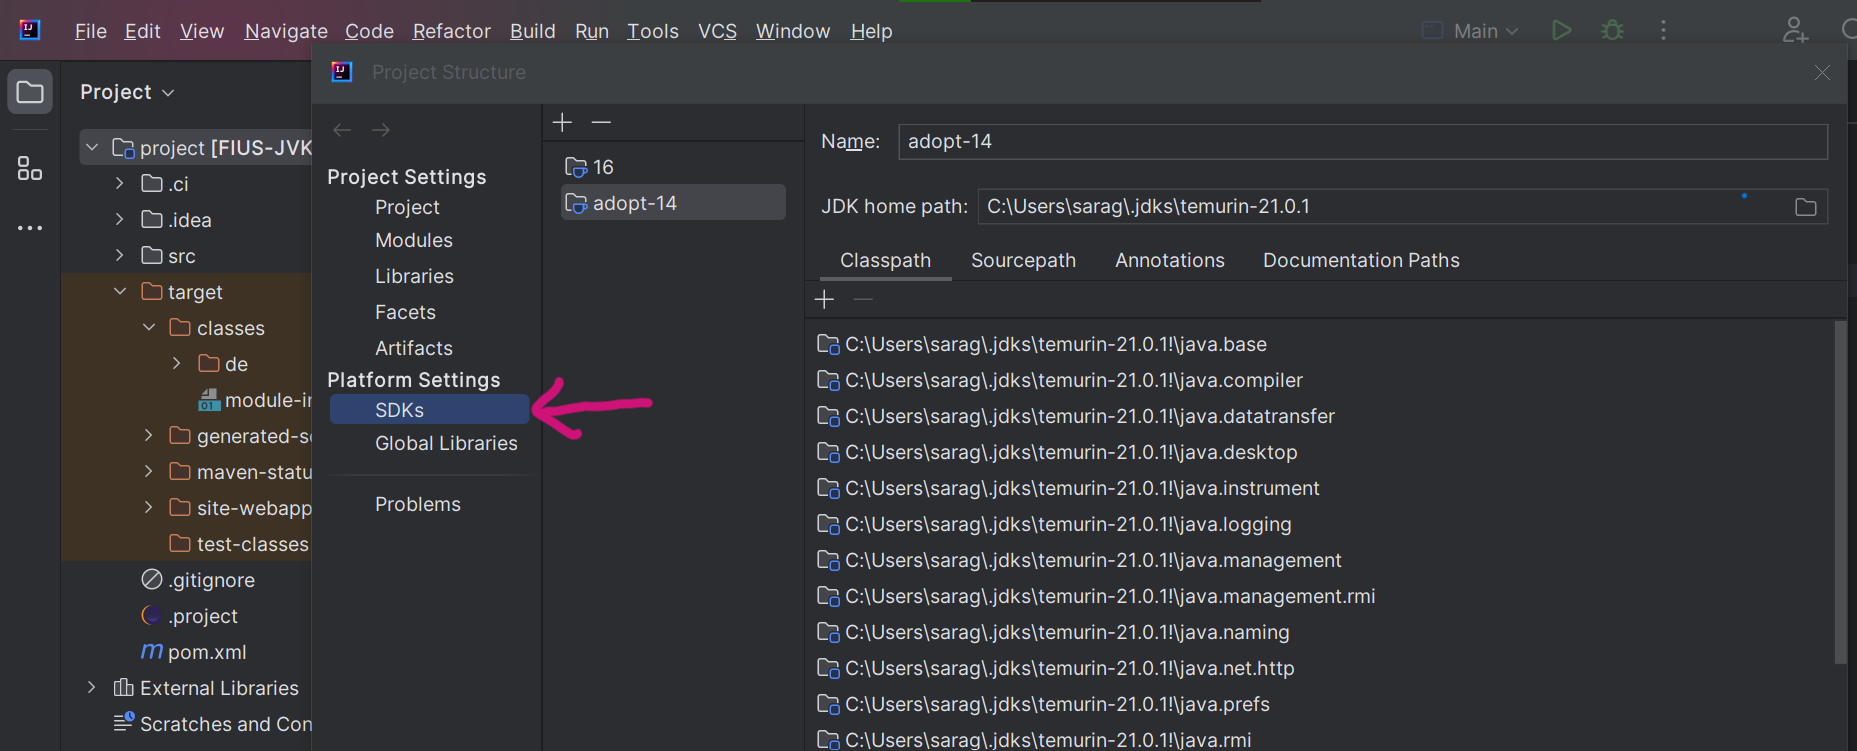
\includegraphics[width=\linewidth]{./figures/IntelliJ JDK.PNG}
\end{center}
\caption{IntelliJ}
\label{fig:IntelliJJDK}
\end{figure}


\begin{figure}[h!]
\begin{center}
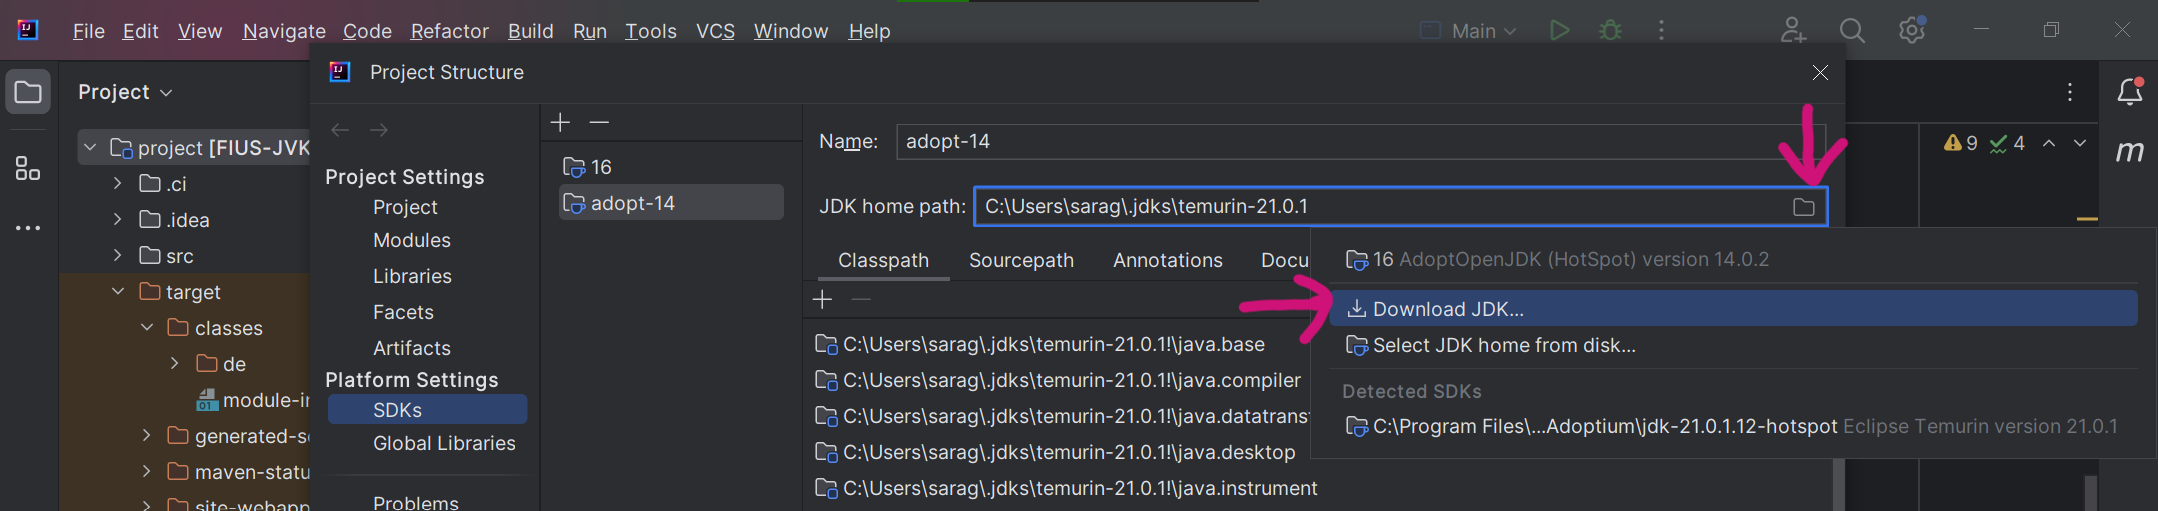
\includegraphics[width=\linewidth]{./figures/IntelliJ JDK 2.PNG}
\end{center}
\caption{IntelliJ}
\label{fig:IntelliJVersion}
\end{figure}

Nun musst du entweder eine schon installierte JDK auswählen oder eine neue installieren. 
Um eine neue JDK zu installieren, musst du die beiden auf Abbildung \ref{fig:IntelliJVersion} markierten Optionen anklicken. 
Jetzt wird sich ein Fenster wie das in Abbildung \ref{fig:javaversion} öffnen.
\newpage

Installiere jetzt die auf der in Abbildung \ref{fig:javaversion} gezeigte Version und füge einen sinnvollen Speicherort hinzu.
\begin{figure}[h]
    \begin{center}
        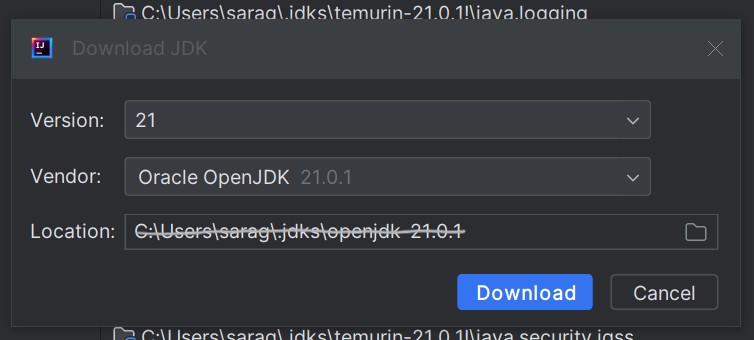
\includegraphics[width=\linewidth]{./figures/IntelliJ JDK 3.PNG}
    \end{center}
    \caption{IntelliJ} 
    \label{fig:javaversion}
\end{figure}

